\documentclass{article}
\usepackage{pgf-pie}
\usepackage{xurl}
\usepackage{listings}
\usepackage{xcolor,colortbl}
\usepackage{makecell}
\usepackage{placeins}
\usepackage{graphicx}
\usepackage{float}
\usepackage{tabstackengine}
\graphicspath{ {./resources/} }

\renewcommand\theadfont{\bfseries}


% 1’eren er sjov fordi I kan gøre lidt ala det med optimerings-opgaven, 
% dokumentere med flotte box-plots osv. Måske kan I finde en hurtigere 
% implementation, at sammenligne med.

% Emne: PriorityQueue i Java
%     Udforsk den inbyggede PriorityQueue i Java
%     Hvorfor er den ikke god? (kan ikke updatere entries, kun linære ændringer (ingen indbygget update() metode))
%     Big O notation
%     Måske en bedre måde at lave den på, eller i hvert fald ideer til forbedringer

% The Dark Side of Java's PriorityQueue
% The Missing Piece in Java's PriorityQueue
\title{Java PriorityQueue Class} 

\author{Anders Jacobsen, Dima Karaush}

% color definition (used for listings)
\definecolor{codegreen}{rgb}{0,0.6,0}
\definecolor{codegray}{rgb}{0.5,0.5,0.5}
\definecolor{codepurple}{rgb}{0.58,0,0.82}
\definecolor{backcolour}{rgb}{0.94,0.94,0.94}

% Designing our listing (Credits to Mutestock : https://github.com/Mutestock)
% He made this style and reviewed an ealier assignment and pointed out that 
% my listing could be improved.
\lstdefinestyle{mystyle}{
    backgroundcolor=\color{backcolour},   
    commentstyle=\color{codegreen},
    keywordstyle=\color{magenta},
    numberstyle=\tiny\color{codegray},
    stringstyle=\color{codepurple},
    basicstyle=\ttfamily,
    breakatwhitespace=false,         
    breaklines=true,                 
    captionpos=b,                    
    keepspaces=true,                 
    numbers=left,                    
    numbersep=5pt,                  
    showspaces=false,                
    showstringspaces=false,
    showtabs=false,                  
    tabsize=2
}

% setting the style to my listings
\lstset{style=mystyle, language=Java}

\begin{document}
\maketitle

\begin{abstract}
    Java's PriorityQueue class has a bottleneck when one needs to update values in the queue.
    Depending on the use and implementation, Java's PriorityQueue can add serious performance 
    issues when accessing the data not using the poll() method.
    When updating a value in the queue, performance can be improved by 99\% in a "worst-case-scenario" compared 
    to Java's PriorityQueue implementation. Implementing your own version might remove this 
    bottleneck from your software. 
\end{abstract}

\section{Introduction}
This article will discuss Java's "build-in" class \lstinline!PriorityQueue!. 
The interest for this topic has grown from an implementation of a weighted graph 
in Java, which we found had a possible shortcoming for our use-case. To update
a value in the queue, we had to use a linear search (loop) through the queue. 
That is fine on a small scale, but the complexity of O(n) can make upscaling a difficult task. 
We believe this can be optimized and that is why this article explores this subject.  

We plan to use Peter Sestofts Mark5 benchmarking techniques from his article 
"Microbenchmarks in Java and C\#" \cite{microbenchmarks7-8} to benchnhmark the two 
PriorityQueue classes. We will do seperate benchmarking with warmup iterations on 
each of the implementations. Afterwards we will explore the data using a Python
Notebook. Then we compare the results to explore our findings. 

The entire project and files can be found on GitHub, the repository is located here 
\url{https://github.com/Cosby1992/UFO_Exam}.


\section{Scope}
This article aims to compare the performance between Java's PriorityQueue
and a PriorityQueue we designed and implemented. The article will only include 
performance comparison for the task to update an Object within. It will not 
compare the enqueueing or dequeueing performance times.

\section{Problem}
\subsection{Background}
% There's no way to find an element in a heap, but to go through all the 
% elements, though pruning (Stop searching if a bigger node is reached) is possible. 
% Therefore a list will be used to make search possible
Java's PriorityQueue is implemented in a heap structure \cite{g4g_pq}, this means that there is no way to quickly find an Object within.
Therefore it is necessary to do a linear iteration through the queue. This is made possible by 
the iterator method inherited in the PriorityQueue class. What we explore is how much faster it would 
be to use binary search \cite{g4g_bs} in a sorted array, where the array is representing a queue instead.  
\subsection{Problem Statement}
\begin{enumerate}
    \item How fast is Java's current implementation, when the task is to update a value within?
    \item How fast is our implementation of PriorityQueue using binary search to find and update a value within?
    \item How do the queue implementations compare in performance?
\end{enumerate}


\section{Analysis}
\subsection{Benchmark Method} % Cosby
This subsection will cover the preparation and execution of the benchmarks.
It will also touch the subject of the timings in the two implementations
of the PriorityQueue class. Peter Sestofts approach to microbenchmarking in 
Java \cite{microbenchmarks7-8} \cite{microbenchmarks5} is used to benchmark the implementations. A combination of Mark5 and Mark3 
benchmarks with minor changes are used to generate the timing results. 
To make benchmarks, a Timer class is necessary. We've designed the a simplest
version possible to avoid interference from calculations in the Timer class.

\begin{lstlisting}[caption={Simple Timer class implementation},label={lst:timerclass}]
    public class Timer {
        private long start;

        public void start() {
            start = System.nanoTime();
        }

        public long step() {
            return System.nanoTime() - start;
        }
    }
\end{lstlisting}

This implementation enables us to process the times as nano seconds after 
the benchmarks and also to easily restart the timer.

In addition to the Timer class we have also implemented a TimerTracker class.
This class only consists of two lists that can contain the warmup and real 
benchmark times, together with a method for writing the obtained times to a CSV\footnote{Comma Separated Values Filestructure} file.
The CSV files will be used to explore the data later.

\begin{lstlisting}[caption={Benchmark iterations}, label={lst:benchmarkiterations}]
    private static void benchmarkPriorityQueue(int warmupIterations, int iterations, TimeTracker tracker) {
        // Printing removed for simplicity
        // Warmup
        for (int i = 0; i < warmupIterations; i++) {
            tracker.addWarmupTime(pQueueRun());
        }
        // Benchmark
        for (int i = 0; i < iterations; i++) {
            tracker.addTime(pQueueRun());
        }
    }
\end{lstlisting}

%How do we measure the times
Measurements in the benchmark is done only on the time it takes to update 
a value in the PriorityQueue. In listing \ref{lst:benchmarkiterations} we run a number of warmup iterations before running the
benchmark. This is to make sure that Java's JIT\footnote{Just In Time} 
compiler has already compiled all the code, before running the benchmarks, as described in Peter Sestofts article \cite{microbenchmarks9-10}. 
In the listing the method \lstinline{pQueueRun()} is running the benchmark, this will be described 
in section \ref{sec:javabenchmark}. The \lstinline{tracker.addTime(long time)} 
simply adds a time to a list that will later be written to a CSV file.

%remember ref to pdf (peter sestoft i disc)
%Something about out Timer, TimerTracker class
%How do we measure the times
%What do we time (ONLY UPDATE)
%Why do we do as we do

\subsection{Update Method} % Dima
There is no method to retrieve a specific node from the queue.
That is why an Iterator is used to run through every node in the queue until a match is found.

\begin{lstlisting}[caption={Finding the node},label={lst:Finding_the_node}]
    Iterator<Node> it = pQueue.iterator();

    timer.start();
    while (it.hasNext()) {
        n = it.next();
        if (count == QUEUE_LENGTH - 1) {
            n.verticeTo = 80085;
            time = timer.step();
            break;
        }
        count++;
    }
\end{lstlisting}

The worst case scenario in a linear search is that our node has the highest 
weight and thus is positioned in the last index of the queue. 
This is also the scenario simulated in our benchmark, by updating the node 
when the check in the code "\lstinline{if (count == QUEUE_LENGTH - 1)}" is true.

Now a thing to note in the code is the way data is inserted in our PriorityQueue. 
Since this part was not the focus of the article, the population of data into the 
queue happens in a linear way, while also moving each element with a lower priority 
one by one. 
Java’s PriorityQueue uses a heap which is a lot faster. This results in our code being 
a lot slower in performance for inserting data.

% Descripe how we implemented our search 
% Descripe that we are NOT using a heap and maybe that our 
% PriorityQueue is MUCH slower than java, in everything but the update method

\subsection{Benchmark of Java's priorityQueue} % Dima
\label{sec:javabenchmark}
%Describe the method for updating (LINEAR WITH ITERATOR)
The initialization and filling of the queue is described in listing \ref{lst:Populating_the_queue}. 
This is an extraction of a code partition from the \lstinline{pQueueRun()} method, 
which is used to measure the benchmark times.

\begin{lstlisting}[caption={Populating the queue},label={lst:Populating_the_queue}]
    PriorityQueue<Node> pQueue = new PriorityQueue<>(QUEUE_LENGTH, nodeComp);

    // Filling the queue with Nodes
    for (int i = 0; i < QUEUE_LENGTH; i++) {
        pQueue.add(new Node(i, i + 1, i));
    }
\end{lstlisting}

In listing \ref{lst:Populating_the_queue} a simple priorityQueue that takes nodes as an object. 
The queue is filled with nodes, the nodes do not require any special values. However a unique 
value is added, so that the nodes are distinguishable.
% Show a description of our numbers
The benchmark is running 5000 times resulting in 5000 data points for exploration. 
On table \ref{tab:regular_times} an overview of the data points are calculated using a Python Notebook.

Looking at the mean and standard deviation on table \ref{tab:regular_times} it is 
visible that the average time for an update is approximately 1046.8 $\mu$s +/- 116.8 $\mu$s. 
The results are visualized using a boxplot in section \ref{sec:comparisson_of_priorityqueues}.

% Here we have zoomed in on a boxplot of the data. \ref{img:boxplotorg}

% \begin{figure}[H]
% \centering
% \label{img:boxplotorg}
% 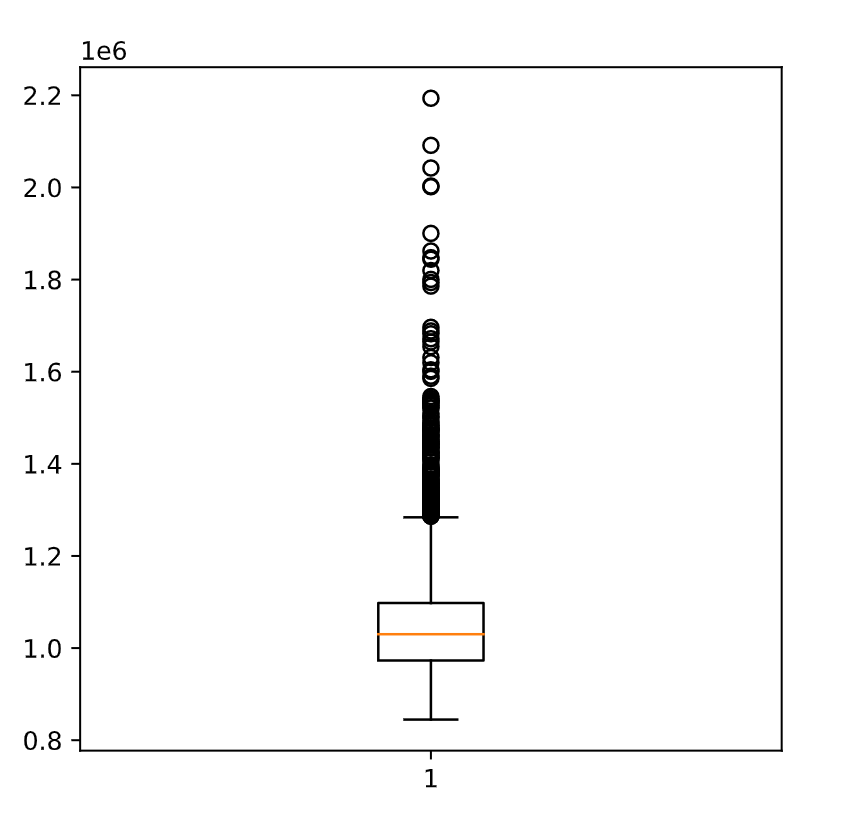
\includegraphics[width=150pt]{boxplotorg}
% \caption{Benchmark boxplot}
% \end{figure}


% Show boxplot of times

\subsection{Benchmark of updatable PriorityQueue} % Cosby
% Describe the method for updating (LINEAR WITH ITERATOR)
The benchmark of the implementation of our PriorityQueue can be seen on 
listing \ref{lst:benchmark_of_selfpq}.

\begin{lstlisting}[caption={Benchmark implmentation on our PriorityQueue},label={lst:benchmark_of_selfpq}]
    private static long pQueueRun() {
        // Initialization removed for simplicity

        timer.start();
        Node n = queue.retrieve(new Node(500, 1000, QUEUE_LENGTH-1));
        n.verticeTo = 101;
        time = timer.step();

        return time;
    }
\end{lstlisting}

As seen listing \ref{lst:benchmark_of_selfpq} the initialization is removed for simplicity in the example. 
So keep in mind that a new queue and timer are initialized every iteration before the benchmark. 
In the example its visible that we use our \lstinline{retrieve()} method to get a specific 
node from the queue. We then mutate a value on the node, and stop the timer. 
Afterwards the time is returned. Later in the benchmark, the returned time is being saved in the
\lstinline{TimerTracker} which writes it to a CSV file. 

Data from the CSV file has been explored using a Python Notebook. 
The results can be found on table \ref{tab:updated_times}. Be aware that the times are measured in microseconds. 

The benchmark completed with an average of 0.409 $\mu$s +/- 0.754 $\mu$s, this can be seen on table \ref{tab:updated_times}.
It is clear that much faster and more stable results from the updated algorithm are achieved. 
In the section \ref{sec:comparisson_of_priorityqueues} a visualization of the data as 
box plots and a comparison of the results will be discussed.


% Show a desciption of our numbers
% Show boxplot of times
\subsection{Comparisson of PriorityQueues} % Dima
\label{sec:comparisson_of_priorityqueues}

\begin{table}[H]
    \parbox{.45\linewidth}{
    \centering
    \begin{tabular}{ |m{2cm}|m{2.5cm}| }
        \hline
        \thead[l]{Count}	                            & 5000	                                    \\
        \cellcolor[HTML]{55FF55}\thead[l]{Mean}	        & \cellcolor[HTML]{55FF55}1046.8 $\mu$s     \\ 
        \cellcolor[HTML]{55FF55}\thead[l]{Std. Dev.}	& \cellcolor[HTML]{55FF55}116.8 $\mu$s	    \\
        \thead[l]{Min}	                                & 844.8	$\mu$s                              \\
        \thead[l]{25\%}	                                & 973.0	$\mu$s                              \\
        \thead[l]{50\%}	                                & 1030.1 $\mu$s                             \\
        \thead[l]{75\%}	                                & 1097.7 $\mu$s                             \\
        \thead[l]{Max}	                                & 2193.6 $\mu$s                             \\
        \hline
    \end{tabular}
        \caption{Key numbers from benchmark} 
        \label{tab:regular_times}
    }
    \hfill
    \parbox{.45\linewidth}{
    \begin{tabular}{ |m{2cm}|m{2.5cm}| }
        \hline
        \thead[l]{Count}                                & 5000                                  \\ 
        \cellcolor[HTML]{55FF55}\thead[l]{Mean}         & \cellcolor[HTML]{55FF55}0.409 $\mu$s  \\  
        \cellcolor[HTML]{55FF55}\thead[l]{Std. Dev.}    & \cellcolor[HTML]{55FF55}0.754 $\mu$s  \\
        \thead[l]{Min}                                  & 0.100 $\mu$s                          \\
        \thead[l]{25\%}                                 & 0.300 $\mu$s                          \\
        \thead[l]{50\%}                                 & 0.300 $\mu$s                          \\ 
        \thead[l]{75\%}                                 & 0.400 $\mu$s                          \\
        \thead[l]{Max}                                  & 31.800 $\mu$s                         \\
        \hline
    \end{tabular}
        \caption{Key numbers from updated benchmark} 
        \label{tab:updated_times}
    }
\end{table}


% How much faster is the method than Javas
The medians are used to calculate the percent increase in performance and the result is a 99.97\% increase. 
%Since the optimized median is only at 300 ns, we can easily calculate that the percent in reduction is at 99.97\%.

% \begin{figure}[ht]
%     \begin{tikzpicture}
%         \pie[rotate = 0, radius = 1.5, text = pin, explode = { 0.5, 0.5 }]
%         {99.970877/Oiginal Time, 0.029123/Optimized Time}
%     \end{tikzpicture}
%     \caption{My Empty Figure}
%     \label{fig:pie_chart}
% \end{figure}
These results can be explained by the complexity of both methods. It is known that a linear operation is defined as O(n) \cite{g4g}.
A binary search has a complexity of O(log n) \cite{g4g-big-o}. 

Now if we compare the results and complexities where n = 500000, which is the same size as our queues in the benchmark.
\begin{table}[H] 
    \centering
    \begin{tabular}{ |l|r|r| }
        \hline
                                & \thead{Results}   & \thead{n = 500000} \\ 
        \hline
        \thead{Linear O(n)}	    & 1030.1 $\mu$s     & 500000           \\
        \thead{Binary O(log n)}	& 0.3 $\mu$s	    & 5.699 	     \\
        \thead{\% difference}	&\cellcolor[HTML]{55FF55} 99.970877 \%	     & \cellcolor[HTML]{55FF55}99.998860 \%	 \\
        \hline
    \end{tabular}
    \caption{Result vs. complexity} 
    \label{tab:ResultNComplexity}
\end{table}

It is visible that our results have increased in performance, with approximately the same amount as expected when looking at the complexity in accordance with the big O notation \cite{g4g-big-o} on table \ref{tab:ResultNComplexity}.
%https://www.geeksforgeeks.org/linear-search/



% Boxplots with comparrison
\begin{figure}[H]
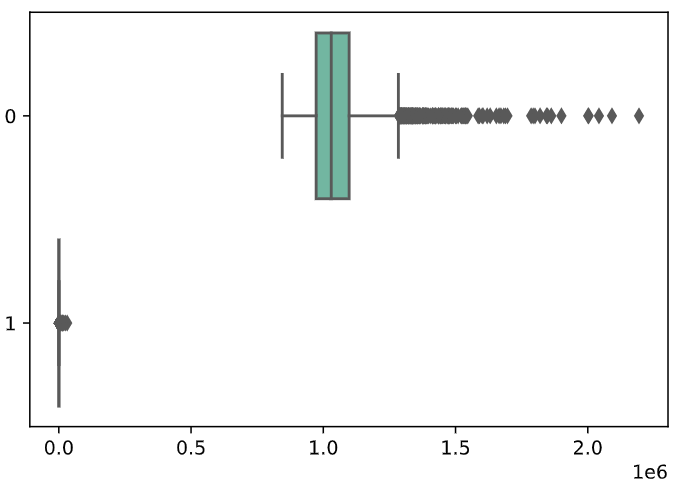
\includegraphics[width=300pt]{boxplot_comparisson}
\caption{Comparisson of the the Priorityqueues}
\label{img:boxplot_comparisson}
\end{figure}

On figure \ref{img:boxplot_comparisson} it is clear that the results is not only faster 
but also a lot more stable. This is visible from the amount of outliers in the two boxplots. 
On the machine which was used for benchmarking, Java's PriorityQueue results end up with a
median of approximately 1 ms with outliers stretching as far as to 2 ms. In comparison to 
our implementation with a median of approximately 300 ns +- 754.987935 ns. The updated 
PriorityQueue reaches much faster and stable results.  

\section{Conclusion} % Cosby
% Something about how much faster our queue is at updating
Updating a value already placed in the queue in Java's PriorityQueue is relatively
fast, with a median of 1.0301 ms searching for a node in a queue with a length of 
500000. Our implementation however is coming in much faster at 300 ns, that is a 99.97\% 
increase in performance. It is not certain that these numbers are precise, since we haven't 
tested it on various machines, only one. But the performance increase does match the expected result 
when comparing the two methods complexity using Big O notation. 
The future of this research could easily be expanded in multiple ways.
It could be tested on multiple machines instead of just one. Furthermore, it could be interesting
to optimize our PriorityQueue to not insert values in a linear fashion. Hereby making it a 
real competitor to the Java standard library implementation.

% Something about how our results are to be taken with a grain of salt, 
% since our priority queue inserts elements linear, therefore it's much 
% slower at everything else in Java's PriorityQueue. 

\bibliographystyle{unsrt}
\bibliography{references}

\end{document}

% \item How fast is Java's current implmentaion, when the task is to update a value within?
% \item How fast is our implementation of PriorityQueue using binary search to find and update a value within?
% \item How do the queues compare in performance?